\documentclass{standalone}
\usepackage{tikz}
\usetikzlibrary{patterns, positioning}
\usepackage[sfdefault]{ClearSans} %% option 'sfdefault' activates Clear Sans as the default text font
\usepackage[T1]{fontenc}

\begin{document}
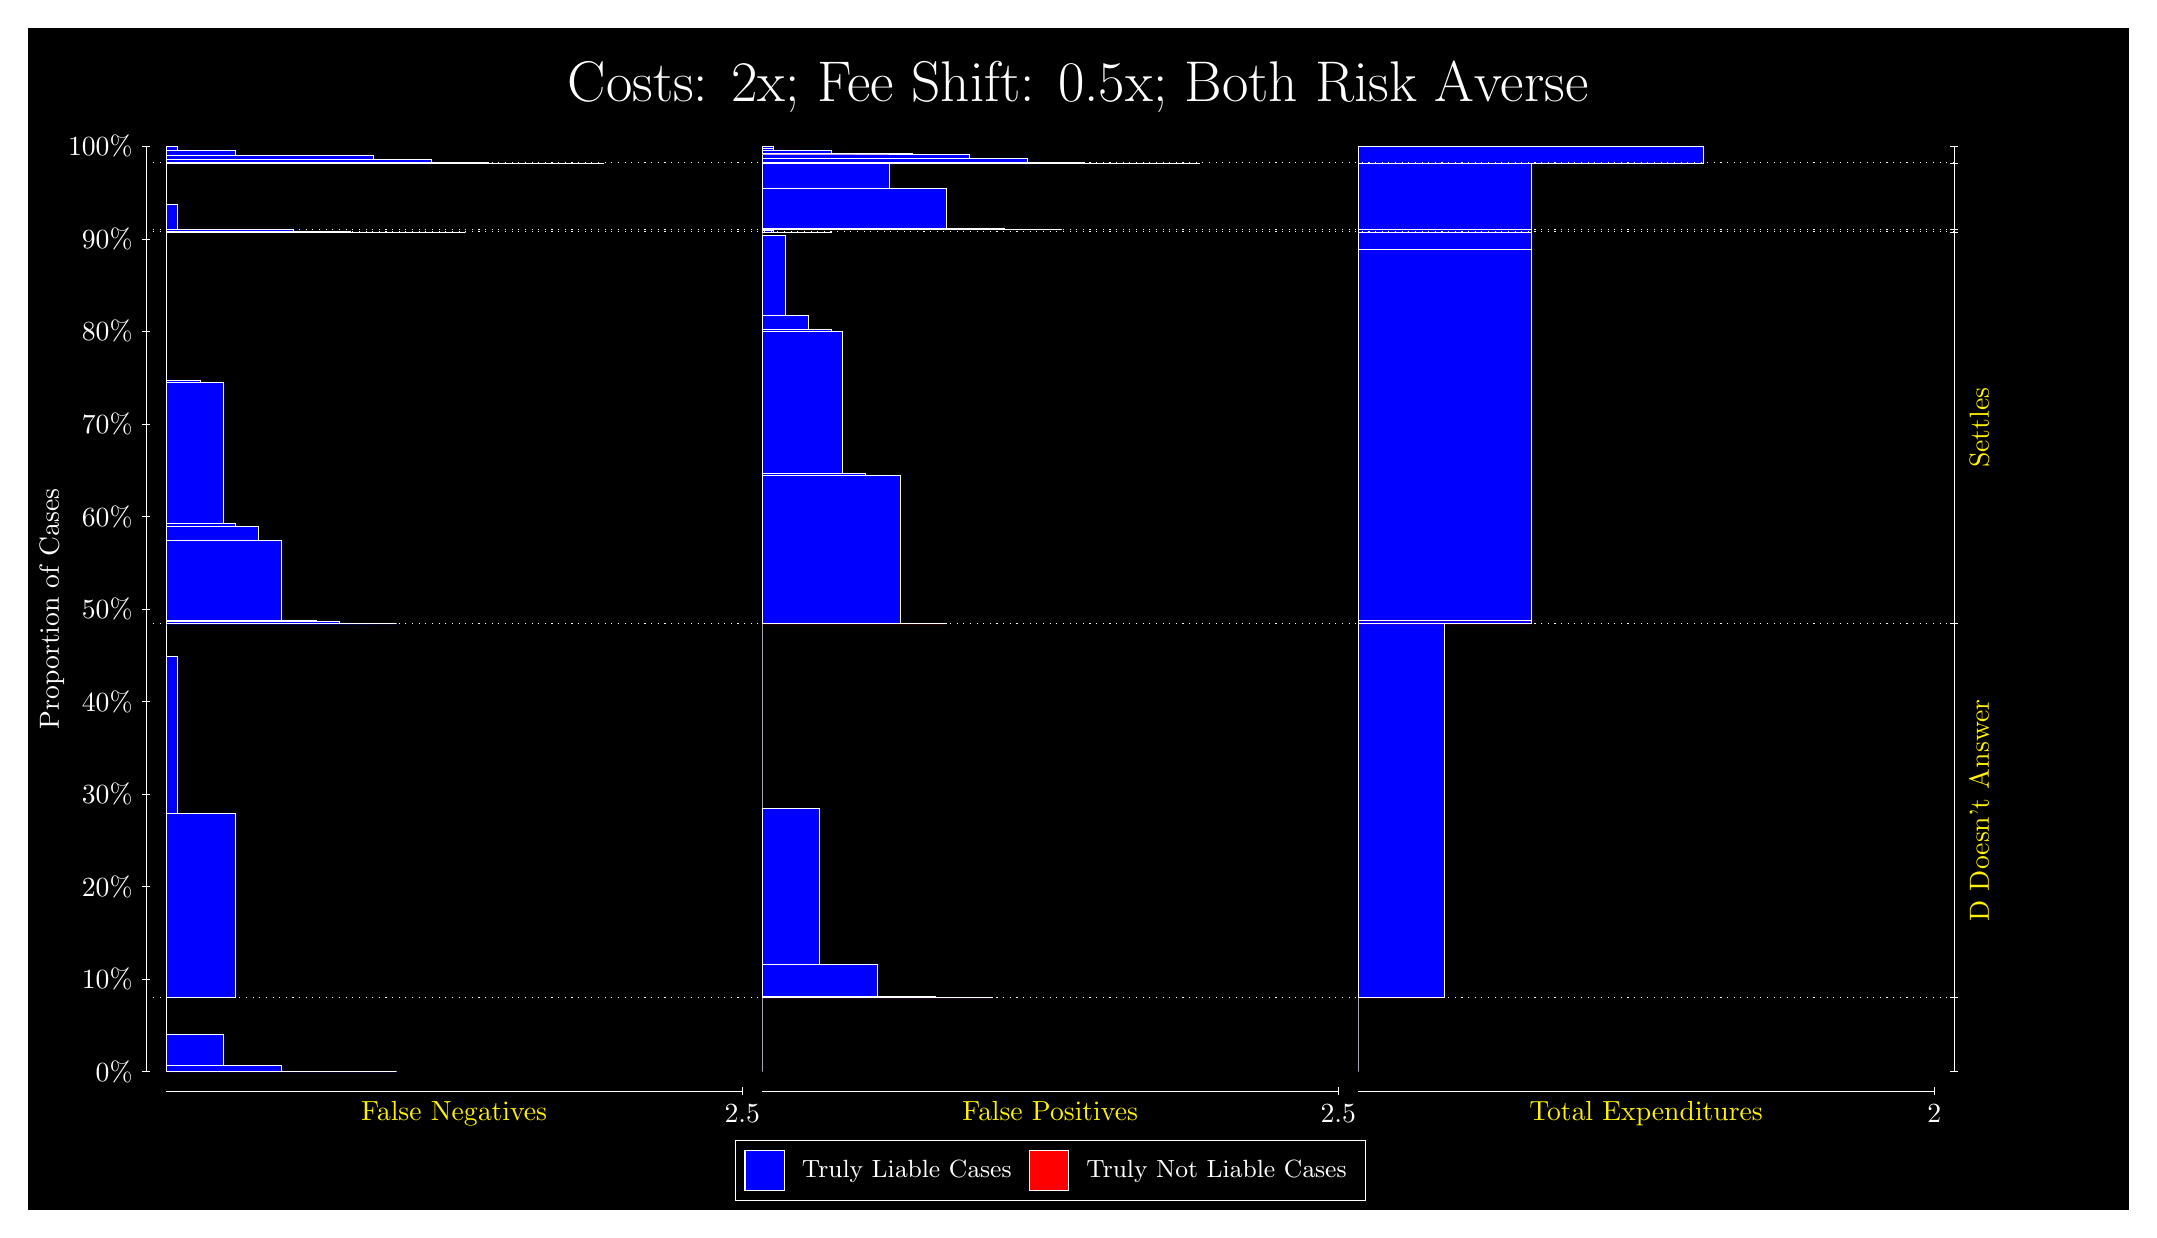
\begin{tikzpicture}
\draw[fill=black] (0,0) rectangle (26.667,15);
\draw[text=white] (0,13.5) rectangle (26.667,15) node[midway] {\huge Costs: 2x; Fee Shift: 0.5x; Both Risk Averse};
\draw[white, very thin] (1.5,1.75) -- (1.5,13.5);
\node[rotate=90, text=white, anchor=center] at (0.3, 7.625) {Proportion of Cases};
\draw[white, very thin] (1.45,1.75) -- (1.55,1.75);
\node[text=white, anchor=east] at (1.45, 1.75) {0\%};
\draw[white, very thin] (1.45,2.925) -- (1.55,2.925);
\node[text=white, anchor=east] at (1.45, 2.925) {10\%};
\draw[white, very thin] (1.45,4.1) -- (1.55,4.1);
\node[text=white, anchor=east] at (1.45, 4.1) {20\%};
\draw[white, very thin] (1.45,5.275) -- (1.55,5.275);
\node[text=white, anchor=east] at (1.45, 5.275) {30\%};
\draw[white, very thin] (1.45,6.45) -- (1.55,6.45);
\node[text=white, anchor=east] at (1.45, 6.45) {40\%};
\draw[white, very thin] (1.45,7.625) -- (1.55,7.625);
\node[text=white, anchor=east] at (1.45, 7.625) {50\%};
\draw[white, very thin] (1.45,8.8) -- (1.55,8.8);
\node[text=white, anchor=east] at (1.45, 8.8) {60\%};
\draw[white, very thin] (1.45,9.975) -- (1.55,9.975);
\node[text=white, anchor=east] at (1.45, 9.975) {70\%};
\draw[white, very thin] (1.45,11.15) -- (1.55,11.15);
\node[text=white, anchor=east] at (1.45, 11.15) {80\%};
\draw[white, very thin] (1.45,12.325) -- (1.55,12.325);
\node[text=white, anchor=east] at (1.45, 12.325) {90\%};
\draw[white, very thin] (1.45,13.5) -- (1.55,13.5);
\node[text=white, anchor=east] at (1.45, 13.5) {100\%};

\draw[white, very thin] (24.457,1.75) -- (24.457,13.5);
\draw[white, very thin] (24.407,1.75) -- (24.507,1.75);
\node[anchor=west] at (24.407, 1.75) {};
\draw[white, very thin] (24.407,2.6898) -- (24.507,2.6898);
\node[anchor=west] at (24.407, 2.6898) {};
\draw[white, very thin] (24.407,7.4399) -- (24.507,7.4399);
\node[anchor=west] at (24.407, 7.4399) {};
\draw[white, very thin] (24.407,12.413) -- (24.507,12.413);
\node[anchor=west] at (24.407, 12.413) {};
\draw[white, very thin] (24.407,12.444) -- (24.507,12.444);
\node[anchor=west] at (24.407, 12.444) {};
\draw[white, very thin] (24.407,13.29) -- (24.507,13.29);
\node[anchor=west] at (24.407, 13.29) {};
\draw[white, very thin] (24.407,13.5) -- (24.507,13.5);
\node[anchor=west] at (24.407, 13.5) {};

\draw[white, very thin, fill=blue] (1.75,1.75) rectangle (4.6775,1.75);
\draw[white, very thin, fill=blue] (1.75,1.75) rectangle (3.9457,1.7506);
\draw[white, very thin, fill=blue] (1.75,1.7506) rectangle (3.2138,1.8252);
\draw[white, very thin, fill=blue] (1.75,1.8252) rectangle (2.4819,2.2205);
\draw[white, very thin, fill=red] (1.75,2.2205) rectangle (1.75,2.2205);
\draw[white, very thin, fill=blue] (1.75,2.2205) rectangle (1.75,2.6898);
\draw[white, very thin, fill=blue] (1.75,2.6898) rectangle (2.6283,5.036);
\draw[white, very thin, fill=blue] (1.75,5.036) rectangle (1.8964,7.0223);
\draw[white, very thin, fill=red] (1.75,7.0223) rectangle (1.75,7.0223);
\draw[white, very thin, fill=blue] (1.75,7.0223) rectangle (1.75,7.4399);
\draw[white, very thin, fill=blue] (1.75,7.4399) rectangle (4.6775,7.4399);
\draw[white, very thin, fill=blue] (1.75,7.4399) rectangle (4.3848,7.4399);
\draw[white, very thin, fill=blue] (1.75,7.4399) rectangle (4.092,7.4399);
\draw[white, very thin, fill=blue] (1.75,7.4399) rectangle (3.9457,7.4732);
\draw[white, very thin, fill=blue] (1.75,7.4732) rectangle (3.6529,7.4819);
\draw[white, very thin, fill=blue] (1.75,7.4819) rectangle (3.3602,7.4833);
\draw[white, very thin, fill=blue] (1.75,7.4833) rectangle (3.2138,8.4988);
\draw[white, very thin, fill=blue] (1.75,8.4988) rectangle (2.921,8.6783);
\draw[white, very thin, fill=blue] (1.75,8.6783) rectangle (2.6283,8.7084);
\draw[white, very thin, fill=blue] (1.75,8.7084) rectangle (2.4819,10.503);
\draw[white, very thin, fill=blue] (1.75,10.503) rectangle (2.1891,10.53);
\draw[white, very thin, fill=blue] (1.75,10.53) rectangle (1.8964,10.534);
\draw[white, very thin, fill=red] (1.75,10.534) rectangle (1.75,10.534);
\draw[white, very thin, fill=blue] (1.75,10.534) rectangle (1.75,12.413);
\draw[white, very thin, fill=blue] (1.75,12.413) rectangle (5.5558,12.413);
\draw[white, very thin, fill=blue] (1.75,12.413) rectangle (4.8239,12.413);
\draw[white, very thin, fill=blue] (1.75,12.413) rectangle (4.092,12.424);
\draw[white, very thin, fill=blue] (1.75,12.424) rectangle (3.3602,12.443);
\draw[white, very thin, fill=blue] (1.75,12.443) rectangle (2.6283,12.444);
\draw[white, very thin, fill=red] (1.75,12.444) rectangle (1.75,12.444);
\draw[white, very thin, fill=blue] (1.75,12.444) rectangle (2.6283,12.447);
\draw[white, very thin, fill=blue] (1.75,12.447) rectangle (1.8964,12.764);
\draw[white, very thin, fill=red] (1.75,12.764) rectangle (1.75,12.764);
\draw[white, very thin, fill=blue] (1.75,12.764) rectangle (1.75,13.29);
\draw[white, very thin, fill=blue] (1.75,13.29) rectangle (7.3123,13.29);
\draw[white, very thin, fill=blue] (1.75,13.29) rectangle (6.5805,13.29);
\draw[white, very thin, fill=blue] (1.75,13.29) rectangle (5.8486,13.293);
\draw[white, very thin, fill=blue] (1.75,13.293) rectangle (5.1167,13.34);
\draw[white, very thin, fill=blue] (1.75,13.34) rectangle (4.8239,13.34);
\draw[white, very thin, fill=blue] (1.75,13.34) rectangle (4.3848,13.384);
\draw[white, very thin, fill=blue] (1.75,13.384) rectangle (4.092,13.384);
\draw[white, very thin, fill=blue] (1.75,13.384) rectangle (3.6529,13.384);
\draw[white, very thin, fill=blue] (1.75,13.384) rectangle (3.3602,13.385);
\draw[white, very thin, fill=blue] (1.75,13.385) rectangle (2.921,13.385);
\draw[white, very thin, fill=blue] (1.75,13.385) rectangle (2.6283,13.385);
\draw[white, very thin, fill=blue] (1.75,13.385) rectangle (2.6283,13.447);
\draw[white, very thin, fill=blue] (1.75,13.447) rectangle (1.8964,13.447);
\draw[white, very thin, fill=blue] (1.75,13.447) rectangle (1.8964,13.495);
\draw[white, very thin, fill=red] (1.75,13.495) rectangle (1.75,13.495);
\draw[white, very thin, fill=blue] (1.75,13.495) rectangle (1.75,13.5);
\draw[white, very thin, fill=red] (9.3189,1.75) rectangle (9.3189,1.75);
\draw[white, very thin, fill=blue] (9.3189,1.75) rectangle (9.3189,2.6898);
\draw[white, very thin, fill=red] (9.3189,2.6898) rectangle (12.246,2.6898);
\draw[white, very thin, fill=blue] (9.3189,2.6898) rectangle (12.246,2.6899);
\draw[white, very thin, fill=blue] (9.3189,2.6899) rectangle (11.515,2.7026);
\draw[white, very thin, fill=blue] (9.3189,2.7026) rectangle (10.783,3.1074);
\draw[white, very thin, fill=blue] (9.3189,3.1074) rectangle (10.051,5.0937);
\draw[white, very thin, fill=blue] (9.3189,5.0937) rectangle (9.3189,7.4399);
\draw[white, very thin, fill=red] (9.3189,7.4399) rectangle (11.661,7.4399);
\draw[white, very thin, fill=blue] (9.3189,7.4399) rectangle (11.661,7.44);
\draw[white, very thin, fill=red] (9.3189,7.44) rectangle (11.368,7.44);
\draw[white, very thin, fill=blue] (9.3189,7.44) rectangle (11.368,7.44);
\draw[white, very thin, fill=red] (9.3189,7.44) rectangle (11.075,7.44);
\draw[white, very thin, fill=blue] (9.3189,7.44) rectangle (11.075,9.319);
\draw[white, very thin, fill=blue] (9.3189,9.319) rectangle (10.929,9.3235);
\draw[white, very thin, fill=blue] (9.3189,9.3235) rectangle (10.636,9.3503);
\draw[white, very thin, fill=blue] (9.3189,9.3503) rectangle (10.344,11.145);
\draw[white, very thin, fill=blue] (9.3189,11.145) rectangle (10.197,11.175);
\draw[white, very thin, fill=blue] (9.3189,11.175) rectangle (9.9044,11.354);
\draw[white, very thin, fill=blue] (9.3189,11.354) rectangle (9.6116,12.37);
\draw[white, very thin, fill=blue] (9.3189,12.37) rectangle (9.4652,12.371);
\draw[white, very thin, fill=blue] (9.3189,12.371) rectangle (9.3189,12.413);
\draw[white, very thin, fill=red] (9.3189,12.413) rectangle (10.197,12.413);
\draw[white, very thin, fill=blue] (9.3189,12.413) rectangle (10.197,12.414);
\draw[white, very thin, fill=blue] (9.3189,12.414) rectangle (9.4652,12.433);
\draw[white, very thin, fill=blue] (9.3189,12.433) rectangle (9.3189,12.444);
\draw[white, very thin, fill=red] (9.3189,12.444) rectangle (13.125,12.444);
\draw[white, very thin, fill=blue] (9.3189,12.444) rectangle (13.125,12.444);
\draw[white, very thin, fill=blue] (9.3189,12.444) rectangle (12.393,12.458);
\draw[white, very thin, fill=blue] (9.3189,12.458) rectangle (11.661,12.969);
\draw[white, very thin, fill=blue] (9.3189,12.969) rectangle (10.929,13.286);
\draw[white, very thin, fill=blue] (9.3189,13.286) rectangle (10.197,13.29);
\draw[white, very thin, fill=red] (9.3189,13.29) rectangle (14.881,13.29);
\draw[white, very thin, fill=blue] (9.3189,13.29) rectangle (14.881,13.29);
\draw[white, very thin, fill=red] (9.3189,13.29) rectangle (14.149,13.29);
\draw[white, very thin, fill=blue] (9.3189,13.29) rectangle (14.149,13.29);
\draw[white, very thin, fill=red] (9.3189,13.29) rectangle (13.417,13.29);
\draw[white, very thin, fill=blue] (9.3189,13.29) rectangle (13.417,13.295);
\draw[white, very thin, fill=red] (9.3189,13.295) rectangle (12.686,13.295);
\draw[white, very thin, fill=blue] (9.3189,13.295) rectangle (12.686,13.343);
\draw[white, very thin, fill=blue] (9.3189,13.343) rectangle (11.954,13.405);
\draw[white, very thin, fill=red] (9.3189,13.405) rectangle (11.661,13.405);
\draw[white, very thin, fill=blue] (9.3189,13.405) rectangle (11.661,13.405);
\draw[white, very thin, fill=blue] (9.3189,13.405) rectangle (11.222,13.406);
\draw[white, very thin, fill=red] (9.3189,13.406) rectangle (10.929,13.406);
\draw[white, very thin, fill=blue] (9.3189,13.406) rectangle (10.929,13.406);
\draw[white, very thin, fill=blue] (9.3189,13.406) rectangle (10.49,13.406);
\draw[white, very thin, fill=blue] (9.3189,13.406) rectangle (10.197,13.449);
\draw[white, very thin, fill=red] (9.3189,13.449) rectangle (10.197,13.449);
\draw[white, very thin, fill=blue] (9.3189,13.449) rectangle (10.197,13.45);
\draw[white, very thin, fill=blue] (9.3189,13.45) rectangle (9.758,13.45);
\draw[white, very thin, fill=blue] (9.3189,13.45) rectangle (9.4652,13.478);
\draw[white, very thin, fill=blue] (9.3189,13.478) rectangle (9.4652,13.497);
\draw[white, very thin, fill=blue] (9.3189,13.497) rectangle (9.3189,13.5);
\draw[white, very thin, fill=red] (16.888,1.75) rectangle (16.888,1.75);
\draw[white, very thin, fill=blue] (16.888,1.75) rectangle (16.888,2.6898);
\draw[white, very thin, fill=red] (16.888,2.6898) rectangle (17.986,2.6898);
\draw[white, very thin, fill=blue] (16.888,2.6898) rectangle (17.986,7.4399);
\draw[white, very thin, fill=red] (16.888,7.4399) rectangle (19.083,7.4399);
\draw[white, very thin, fill=blue] (16.888,7.4399) rectangle (19.083,7.476);
\draw[white, very thin, fill=red] (16.888,7.476) rectangle (19.083,7.476);
\draw[white, very thin, fill=blue] (16.888,7.476) rectangle (19.083,12.198);
\draw[white, very thin, fill=red] (16.888,12.198) rectangle (19.083,12.198);
\draw[white, very thin, fill=blue] (16.888,12.198) rectangle (19.083,12.413);
\draw[white, very thin, fill=red] (16.888,12.413) rectangle (19.083,12.413);
\draw[white, very thin, fill=blue] (16.888,12.413) rectangle (19.083,12.444);
\draw[white, very thin, fill=red] (16.888,12.444) rectangle (19.083,12.444);
\draw[white, very thin, fill=blue] (16.888,12.444) rectangle (19.083,13.29);
\draw[white, very thin, fill=red] (16.888,13.29) rectangle (21.279,13.29);
\draw[white, very thin, fill=blue] (16.888,13.29) rectangle (21.279,13.5);
\draw[white, dotted] (1.5,2.6898) -- (24.457,2.6898);
\draw[white, dotted] (1.5,7.4399) -- (24.457,7.4399);
\draw[white, dotted] (1.5,12.413) -- (24.457,12.413);
\draw[white, dotted] (1.5,12.444) -- (24.457,12.444);
\draw[white, dotted] (1.5,13.29) -- (24.457,13.29);
\draw[white, very thin] (1.75,1.5) -- (9.0689,1.5);
\node[text=yellow, anchor=north] at (5.4094, 1.5) {False Negatives};
\draw[white, very thin] (9.0689,1.45) -- (9.0689,1.55);
\node[text=white, anchor=north] at (9.0689, 1.45) {2.5};

\draw[white, very thin] (9.3189,1.5) -- (16.638,1.5);
\node[text=yellow, anchor=north] at (12.978, 1.5) {False Positives};
\draw[white, very thin] (16.638,1.45) -- (16.638,1.55);
\node[text=white, anchor=north] at (16.638, 1.45) {2.5};

\draw[white, very thin] (16.888,1.5) -- (24.207,1.5);
\node[text=yellow, anchor=north] at (20.547, 1.5) {Total Expenditures};
\draw[white, very thin] (24.207,1.45) -- (24.207,1.55);
\node[text=white, anchor=north] at (24.207, 1.45) {2};


\node[text=yellow, centered, rotate=90] at (24.777, 5.0649) {D Doesn't Answer};
\node[text=yellow, centered, rotate=90] at (24.777, 9.9266) {Settles};




\draw (12.978300999999998,1.5) node[draw=none] (baseCoordinate) {};
\begin{scope}[align=center]
        \matrix[scale=0.5, draw=white, below=0.5cm of baseCoordinate, nodes={draw}, column sep=0.1cm]{
            \node[rectangle, draw, minimum width=0.5cm, minimum height=0.5cm, fill=blue] {}; &
            \node[draw=none, font=\small, text=white] (B) {Truly Liable Cases}; &
            \node[rectangle, draw, minimum width=0.5cm, minimum height=0.5cm, fill=red] {}; &
            \node[draw=none, font=\small, text=white] (B) {Truly Not Liable Cases}; \\
            };
\end{scope}

\end{tikzpicture}
\end{document}